   \begin{figure}[h]
        \centering
		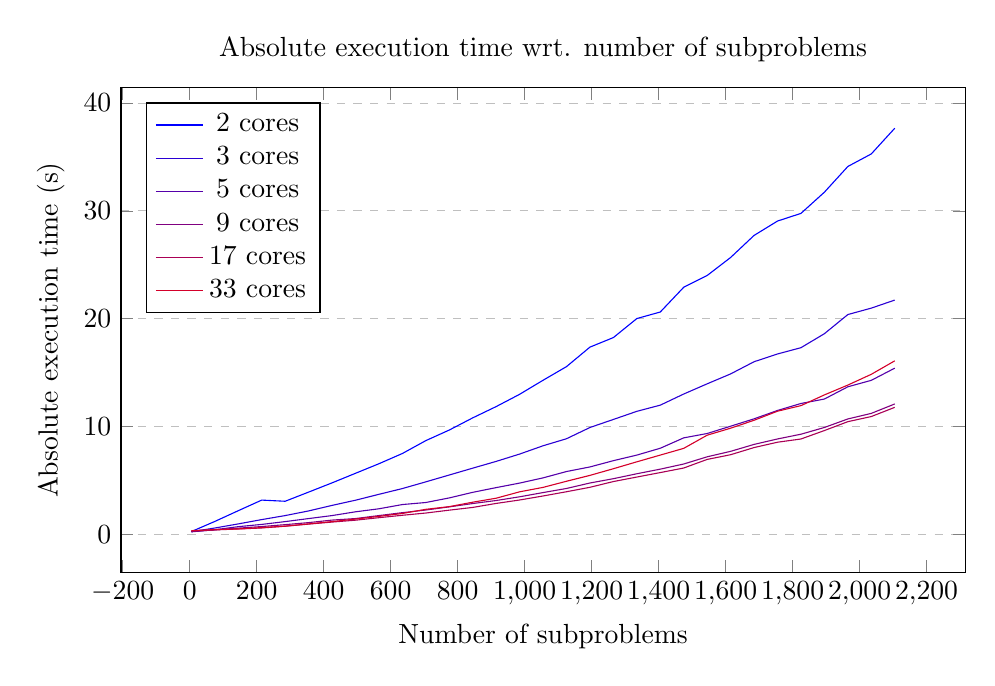
\begin{tikzpicture}
		\begin{axis}[
			title={Absolute execution time wrt. number of subproblems},
			xlabel={Number of subproblems},
			ylabel={Absolute execution time (s)},
			%xmin=0, xmax=0.25,
			%ymin=10.00, ymax=100000.00,
			%ymode=log,
			%xtick={0,0.05,0.1,0.15,0.2,0.25},
			%ytick={0,20,40,60,80,100},
			%yticklabel=$\pgfmathprintnumber{\tick}\%$,
			legend pos=north west,
			ymajorgrids=true,
			grid style=dashed,
			xticklabel style={/pgf/number format/fixed},
			width = 350,
			height = 220
		]




\addplot[color=red!0.0!blue,line width=0.4pt] coordinates {
(5,0.2362961769104004)(75,1.1755552291870117)(145,2.173146963119507)(215,3.157050848007202)(285,3.0487685203552246)(355,3.8985092639923096)(425,4.755660533905029)(495,5.643772602081299)(565,6.531620502471924)(635,7.4814841747283936)(705,8.676511764526367)(775,9.6584312915802)(845,10.788349628448486)(915,11.835201978683472)(985,12.97413420677185)(1055,14.27720332145691)(1125,15.543988466262817)(1195,17.353617668151855)(1265,18.240656852722168)(1335,20.005002737045288)(1405,20.61204719543457)(1475,22.910298585891724)(1545,24.000704765319824)(1615,25.671855211257935)(1685,27.71861171722412)(1755,29.05149006843567)(1825,29.763449668884277)(1895,31.731281280517578)(1965,34.11725568771362)(2035,35.28141164779663)(2105,37.66511368751526)
}node[pos=0.8](endofplotsquare){} ;
\addlegendentry{2 cores}
\addplot[color=red!16.666666666666668!blue,line width=0.4pt] coordinates {
(5,0.22471952438354492)(75,0.5662057399749756)(145,0.9474582672119141)(215,1.348191499710083)(285,1.7202212810516357)(355,2.151851177215576)(425,2.665273904800415)(495,3.1462738513946533)(565,3.693495988845825)(635,4.227936029434204)(705,4.85132622718811)(775,5.485703945159912)(845,6.121047019958496)(915,6.748381614685059)(985,7.428805828094482)(1055,8.197736501693726)(1125,8.851788997650146)(1195,9.894617795944214)(1265,10.641643524169922)(1335,11.394659757614136)(1405,11.9686861038208)(1475,13.001048803329468)(1545,13.947997093200684)(1615,14.866320371627808)(1685,15.998363256454468)(1755,16.718042373657227)(1825,17.30029273033142)(1895,18.59991478919983)(1965,20.375839233398438)(2035,20.972047805786133)(2105,21.719709873199463)
}node[pos=0.8](endofplotsquare){} ;
\addlegendentry{3 cores}
\addplot[color=red!33.333333333333336!blue,line width=0.4pt] coordinates {
(5,0.21304702758789062)(75,0.40426206588745117)(145,0.6919465065002441)(215,0.8999366760253906)(285,1.161741018295288)(355,1.4429419040679932)(425,1.7209069728851318)(495,2.0703799724578857)(565,2.3511414527893066)(635,2.743969202041626)(705,2.93356990814209)(775,3.3594651222229004)(845,3.8780977725982666)(915,4.315030574798584)(985,4.735558748245239)(1055,5.218811988830566)(1125,5.80847954750061)(1195,6.234036207199097)(1265,6.816247940063477)(1335,7.3333940505981445)(1405,7.969827890396118)(1475,8.932463884353638)(1545,9.336983680725098)(1615,10.014135122299194)(1685,10.699220180511475)(1755,11.475051641464233)(1825,12.123208999633789)(1895,12.535733938217163)(1965,13.671947479248047)(2035,14.27146577835083)(2105,15.399876117706299)
}node[pos=0.8](endofplotsquare){} ;
\addlegendentry{5 cores}
\addplot[color=red!50.0!blue,line width=0.4pt] coordinates {
(5,0.23718547821044922)(75,0.39684247970581055)(145,0.5541701316833496)(215,0.7023584842681885)(285,0.8778998851776123)(355,1.0677170753479004)(425,1.3016605377197266)(495,1.4439446926116943)(565,1.7219109535217285)(635,1.9910361766815186)(705,2.2353708744049072)(775,2.528398036956787)(845,2.8381338119506836)(915,3.1183969974517822)(985,3.463233470916748)(1055,3.8552088737487793)(1125,4.2365453243255615)(1195,4.743107080459595)(1265,5.144285202026367)(1335,5.602648973464966)(1405,6.029825448989868)(1475,6.506726264953613)(1545,7.1754631996154785)(1615,7.681975603103638)(1685,8.325080871582031)(1755,8.830584049224854)(1825,9.272136449813843)(1895,9.895843505859375)(1965,10.687816381454468)(2035,11.204007387161255)(2105,12.079752206802368)
}node[pos=0.8](endofplotsquare){} ;
\addlegendentry{9 cores}
\addplot[color=red!66.66666666666667!blue,line width=0.4pt] coordinates {
(5,0.2891275882720947)(75,0.3904001712799072)(145,0.4757850170135498)(215,0.5699207782745361)(285,0.7323768138885498)(355,0.9299347400665283)(425,1.118117332458496)(495,1.292304515838623)(565,1.525442361831665)(635,1.748434066772461)(705,1.957042932510376)(775,2.223759651184082)(845,2.476705551147461)(915,2.8478481769561768)(985,3.1665890216827393)(1055,3.5390067100524902)(1125,3.9331343173980713)(1195,4.345015525817871)(1265,4.87886118888855)(1335,5.296087265014648)(1405,5.711444616317749)(1475,6.134087324142456)(1545,6.932433128356934)(1615,7.369121313095093)(1685,8.03252911567688)(1755,8.528788566589355)(1825,8.827685832977295)(1895,9.611763715744019)(1965,10.435662269592285)(2035,10.911863565444946)(2105,11.763577699661255)
}node[pos=0.8](endofplotsquare){} ;
\addlegendentry{17 cores}
\addplot[color=red!83.33333333333333!blue,line width=0.4pt] coordinates {
(5,0.32294368743896484)(75,0.41986513137817383)(145,0.48233509063720703)(215,0.6048417091369629)(285,0.7414553165435791)(355,0.9482111930847168)(425,1.16239333152771)(495,1.3949286937713623)(565,1.645319938659668)(635,1.9154088497161865)(705,2.3016510009765625)(775,2.5509541034698486)(845,2.9621360301971436)(915,3.3325388431549072)(985,3.925122022628784)(1055,4.336254119873047)(1125,4.905707359313965)(1195,5.449917554855347)(1265,6.069330453872681)(1335,6.710622310638428)(1405,7.333817720413208)(1475,7.9586451053619385)(1545,9.180939674377441)(1615,9.829682111740112)(1685,10.564534664154053)(1755,11.407931804656982)(1825,11.923769474029541)(1895,12.91983437538147)(1965,13.831814765930176)(2035,14.831673383712769)(2105,16.079890727996826)
}node[pos=0.8](endofplotsquare){} ;
\addlegendentry{33 cores}



		\end{axis}
		\end{tikzpicture}
		%\vspace{-18pt}
		\caption[Absolute execution time wrt. number small-hard subproblems]{Runtime on paralell small-hard subproblems, for different numbers of cores and subprobems}
		\label{fig:performance_graph2}
    \end{figure}
